\documentclass[11pt,a4paper]{article}

\usepackage{titling}
\usepackage[hidelinks]{hyperref}
\usepackage{graphicx}
\usepackage{grffile}
\usepackage{float}
\usepackage{geometry}
\usepackage{listings}

\newcommand{\subtitle}[1]{
  \posttitle{
    \par\end{center}
    \begin{center}\large#1\end{center}
    \vskip0.5em}
}

\begin{document}
\title{Web Application User Manual}
\subtitle{ Git: \url{https://github.com/CodingInfinity/Benchmark-Service-Documentation} \\ GitHub Organisation: \url{https://github.com/CodingInfinity}}
\begin{figure}
			\centering
			
\includegraphics[height=230px]{../Images/CodingInfinity.png}
\end{figure}
\author{
	\textbf{The Client:} \\
	Ms Vreda Pieterse  \\
	Department of Computer Science \\
	University Of Pretoria
	\\
	\\
	\textbf{The Team:} \\
	Andrew Broekman		\emph{11089777}	\\
	Brenton Watt		\emph{14032644}	\\
	Fabio Loreggian		\emph{14040426}	\\
	Reinhardt Cromhout	\emph{14009936}	\\
}
\date{\textbf{September 2016}}

\maketitle
\thispagestyle{empty}
\pagebreak

\tableofcontents
\pagebreak
\section{Introduction}
This is the user manual for the Web Application. It gives a detailed guide surrounding individual how to
navigate and use each part of the system.

\subsection{System Overview}
In a broad sense, the web application acts as a front end to the benchmarking service that makes up the 
overall system, the web application serves as a means to communicate with backend in terms of uploading
datasets and algorithms, creating experiments, viewing results and managing account details.

\subsection{System Configuration}
As seen in Figure \ref{fig:config} the system as a whole compromises of a front end, coded in Angular2,
a backend coded in Java, A messaging platform coded in ActiveMQ, and a Instrumentation Application coded
in C++.
\begin{figure}[H]
	\begin{center}
		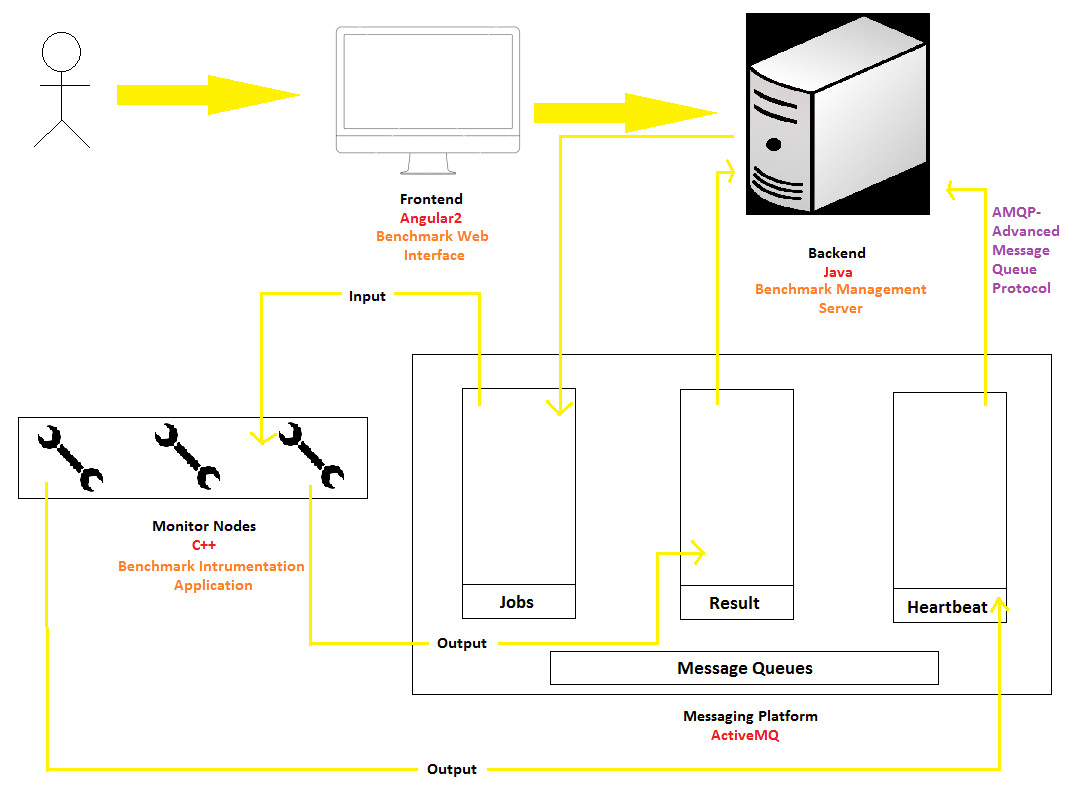
\includegraphics[scale=0.5]{../Images/User Manual/System Configuration.png}
		\caption{System Configuration}
		\label{fig:config}
	\end{center}  
\end{figure}
  
\subsection{Installation}
The system has only thoroughly been tested to work on the Google Chrome browser, for optimal usage of the 
web application system it is recommended that the user make use of Google Chrome, the default installation
setting of Chrome will be sufficient. At the time of writing the IP address for the system is 137.215.40.157
i.e the service can be accessed by directing the users browser to 137.215.40.157, this is an internal 
University of Pretoria(UP) IP address and as such can only be accessed from within the UP firewall. The 
installation of the backend and the monitoring system is discussed in further detail in the installation manual.
\clearpage
\section{Registration}
Upon starting up of the application and navigating to the home page, the user will be met with the screen seen in 
Figure \ref{fig:landPage}.
\begin{figure}[H]
	\begin{center}
		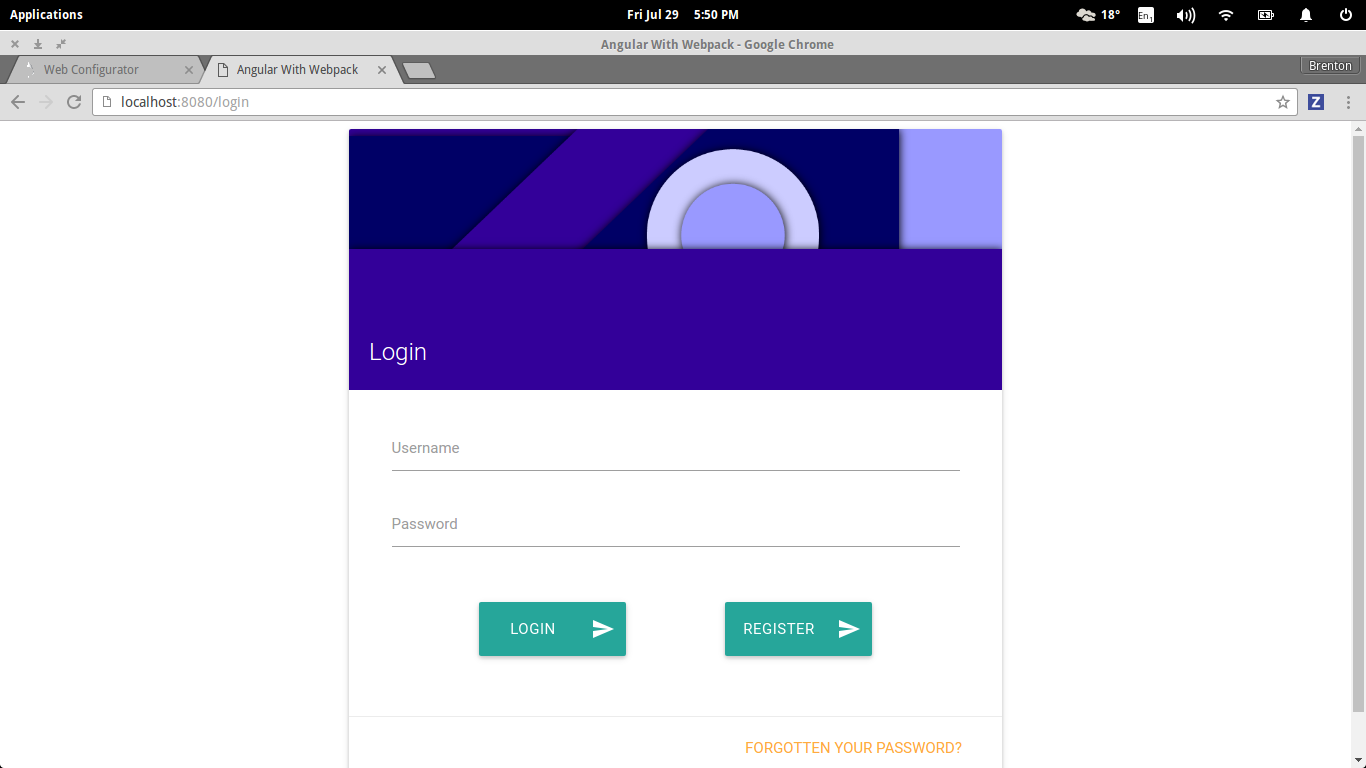
\includegraphics[scale=0.3]{../Images/User Manual/Landing Page.png}
		\caption{Landing Page}
		\label{fig:landPage}
	\end{center}  
\end{figure}

\clearpage
If the user has never made use of the system before, they should register themselves. Clicking on the "Register"
button will direct the user to the page seen in Figure \ref{fig:regPage}.
\begin{figure}[H]
	\begin{center}
		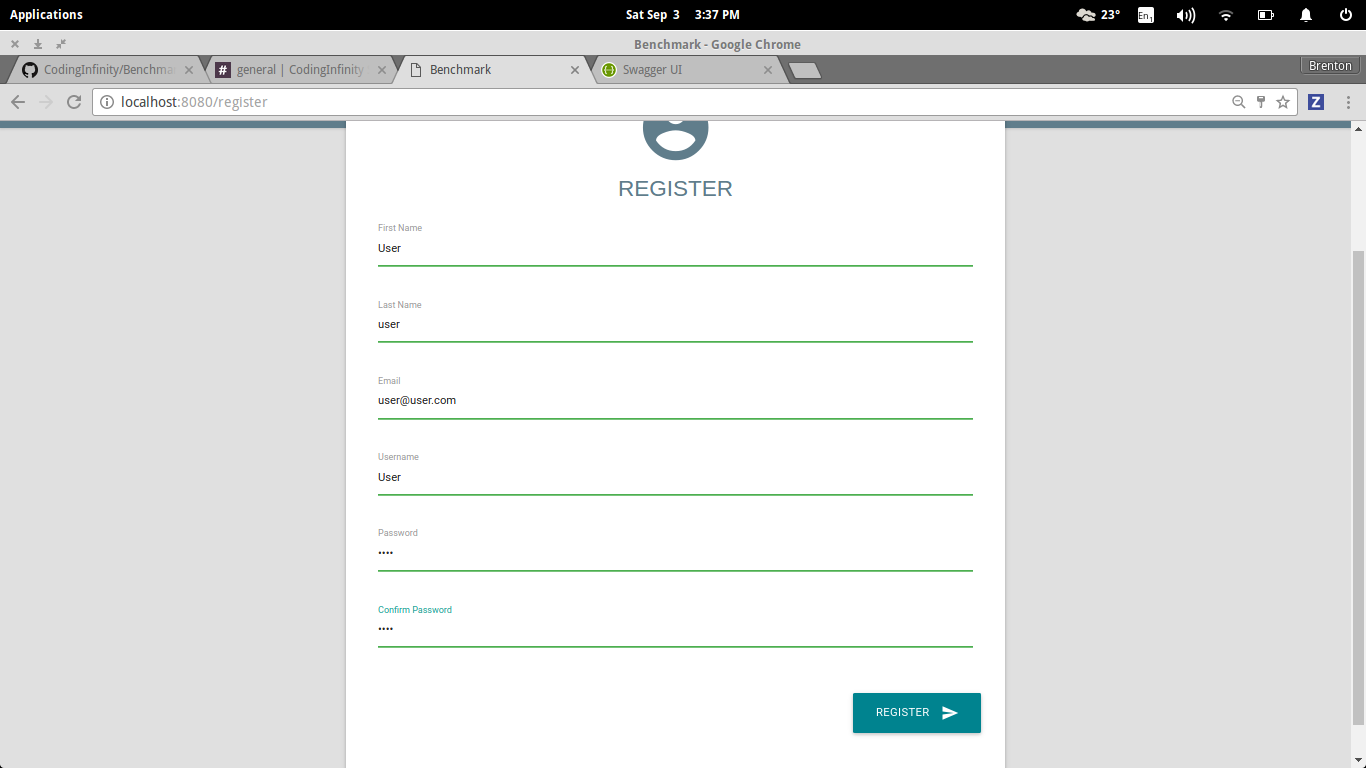
\includegraphics[scale=0.3]{../Images/User Manual/Registration Page.png}
		\caption{Registration Page}
		\label{fig:regPage}
	\end{center}  
\end{figure}

The user will then need to fill in their details accordingly. Once they have done this, they should click the "Submit" 
button. The user will then receive an email address at the address provided with a link that will allow them to activate
their account.
 
\clearpage When they click on the link they will arrive at a page as seen in Figure \ref{fig:activatePage}.
\begin{figure}[H]
	\begin{center}
		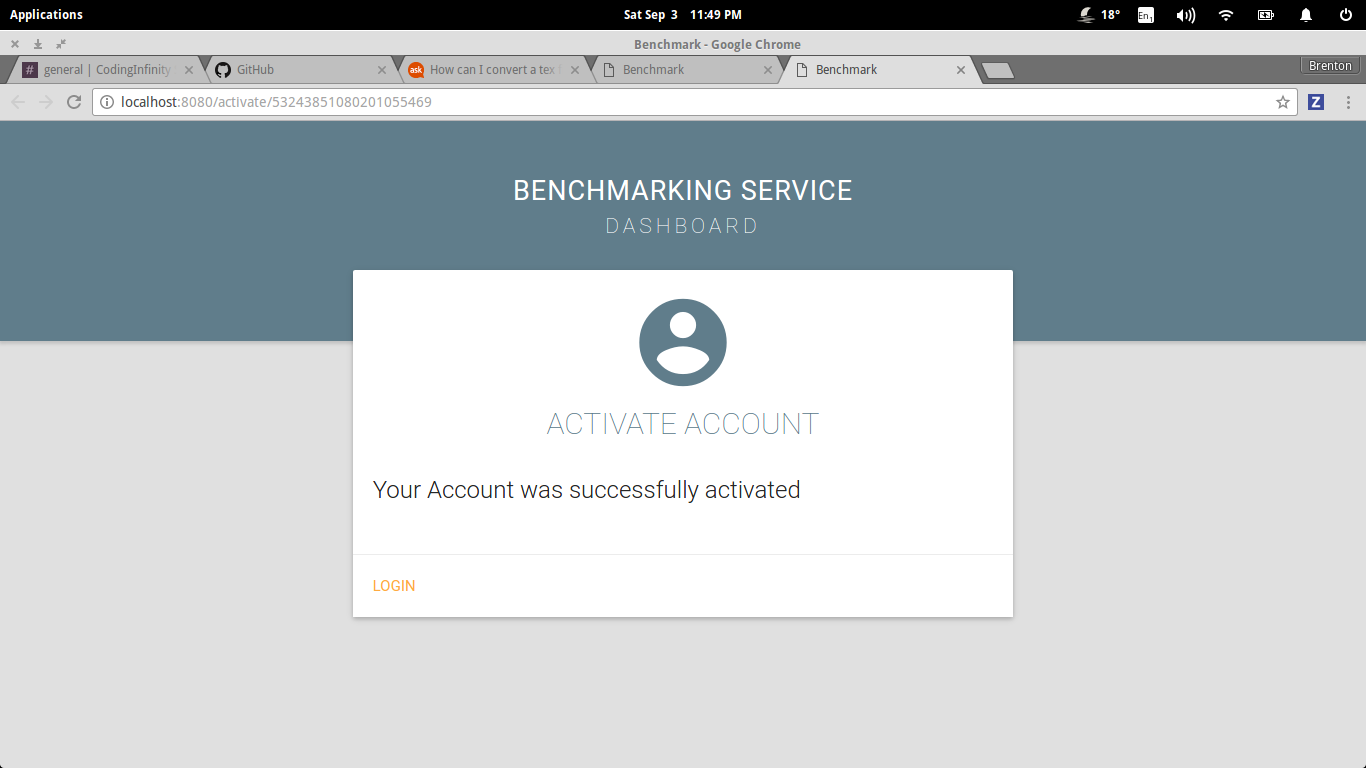
\includegraphics[scale=0.3]{../Images/User Manual/Activation Page.png}
		\caption{Activation Page}
		\label{fig:activatePage}
	\end{center}  
\end{figure}

\clearpage
\section{Sign In}
Once the user has registered and activated an account as detailed in the previous section or upon returning to the application,
they will be able to sign in by filling in their details as seen in Figure \ref{fig:signPage}.
\begin{figure}[H]
	\begin{center}
		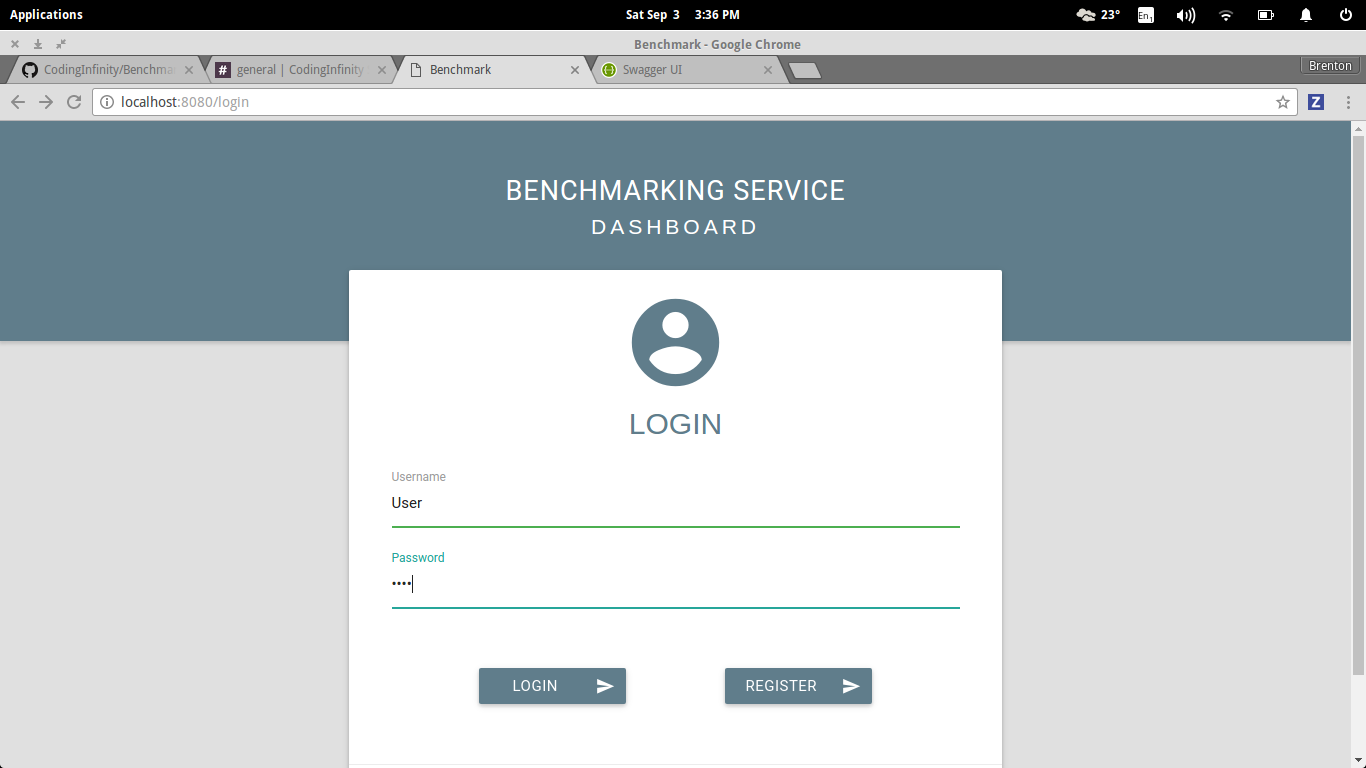
\includegraphics[scale=0.3]{../Images/User Manual/Sign in Page.png}
		\caption{Signing in}
		\label{fig:signPage}
	\end{center}  
\end{figure}

\clearpage
\section{Home}
Upon signing in, the user will arrive at the home page as seen in Figure \ref{fig:homePage}. From this page the user will be able 
to navigate throughout the application.
\begin{figure}[H]
	\begin{center}
		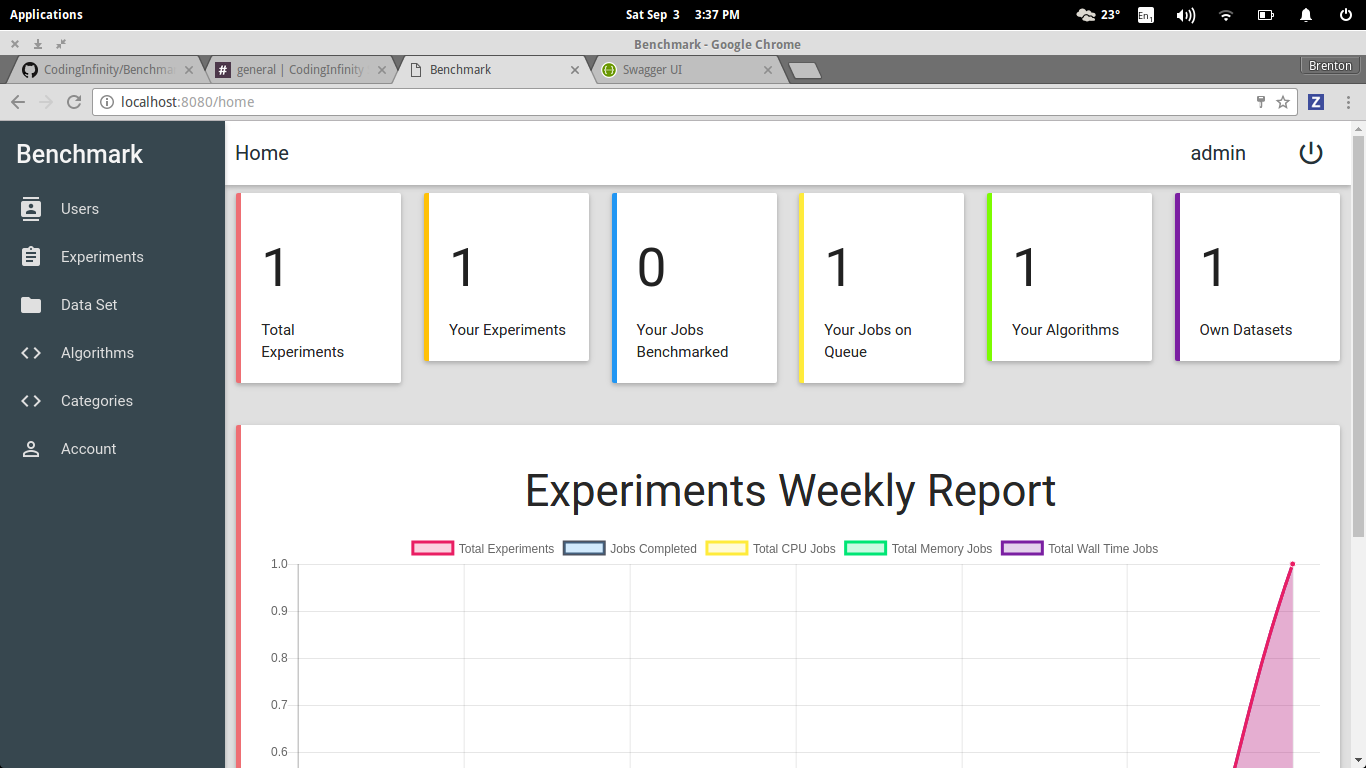
\includegraphics[scale=0.3]{../Images/User Manual/Home Page.png}
		\caption{Home Page}
		\label{fig:homePage}
	\end{center}  
\end{figure}
\clearpage
\section{Edit Profile}
In order to edit ones profile, click on the Account tab in the navigation bar and a drop down list will appear as seen in Figure \ref{fig:AccountPage}.
\begin{figure}[H]
	\begin{center}
		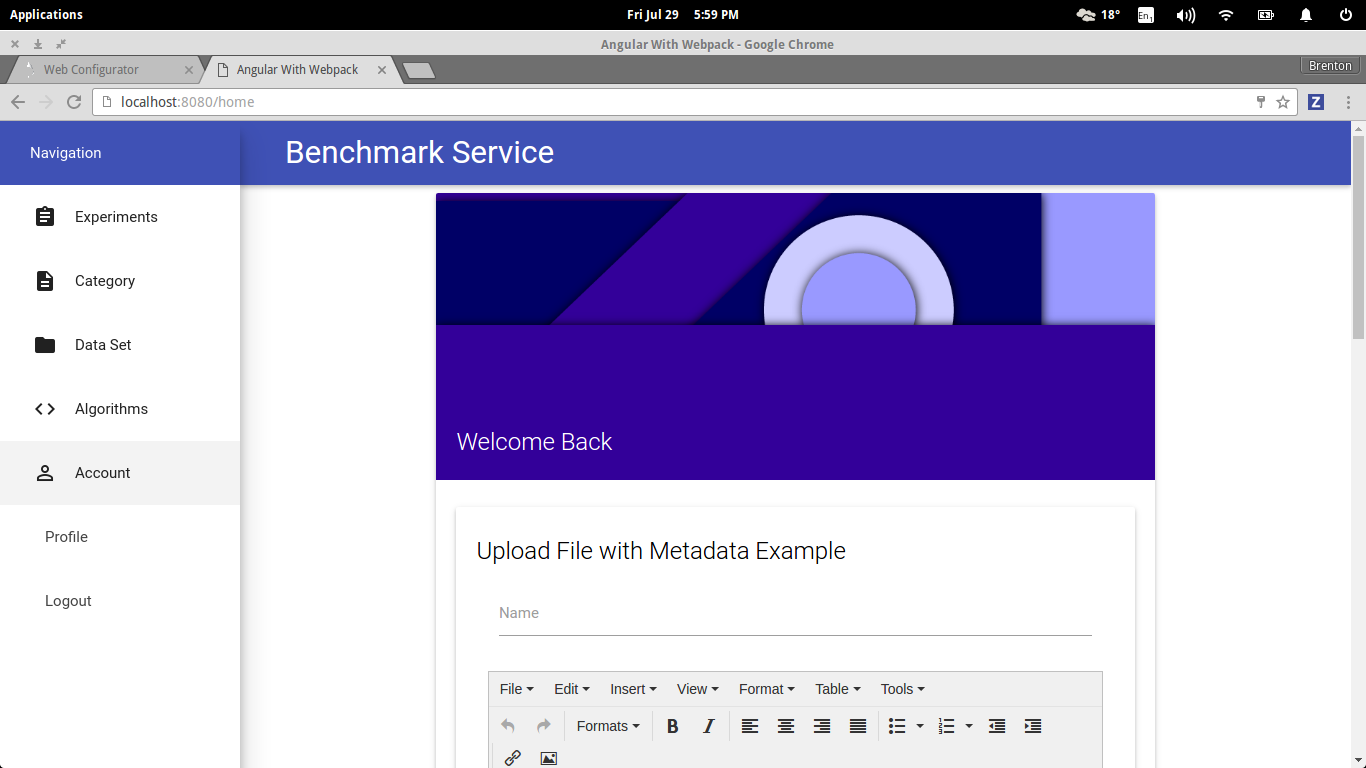
\includegraphics[scale=0.3]{../Images/User Manual/Account Page.png}
		\caption{Home Page with Account menu options extended.}
		\label{fig:AccountPage}
	\end{center}  
\end{figure}
\clearpage From there, click on the "Profile" option, which will take you to the Profile page as seen in Figure \ref{fig:ProfilePage}.
\begin{figure}[H]
	\begin{center}
		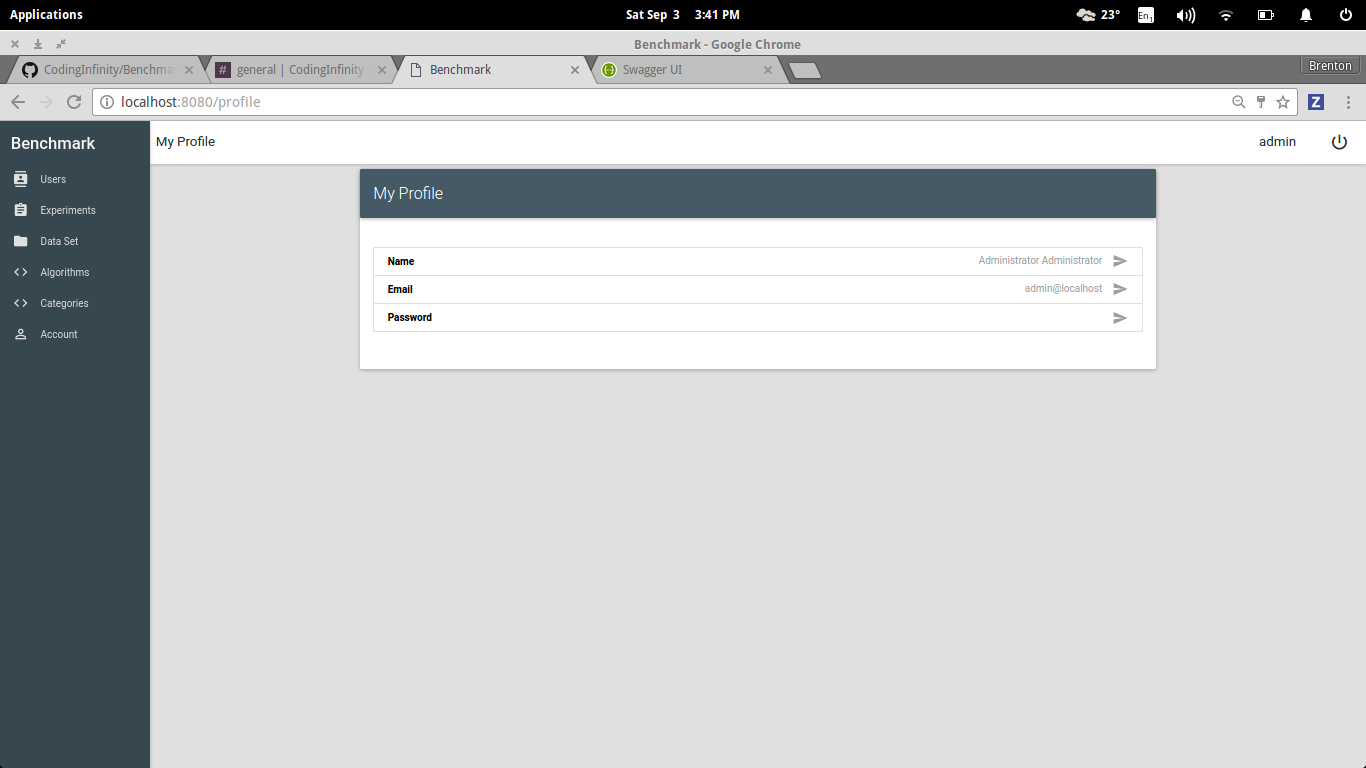
\includegraphics[scale=0.3]{../Images/User Manual/Profile Page.png}
		\caption{Profile Page}
		\label{fig:ProfilePage}
	\end{center}  
\end{figure}
\clearpage
From here, the user can edit any of the options available by clicking on the desired option and filling in the details as seen in
Figures \ref{fig:ProfilePage1}, \ref{fig:ProfilePage2}, \ref{fig:ProfilePage3}. Upon filling in the details, click the "Edit" button.
\begin{figure}[H]
	\begin{center}
		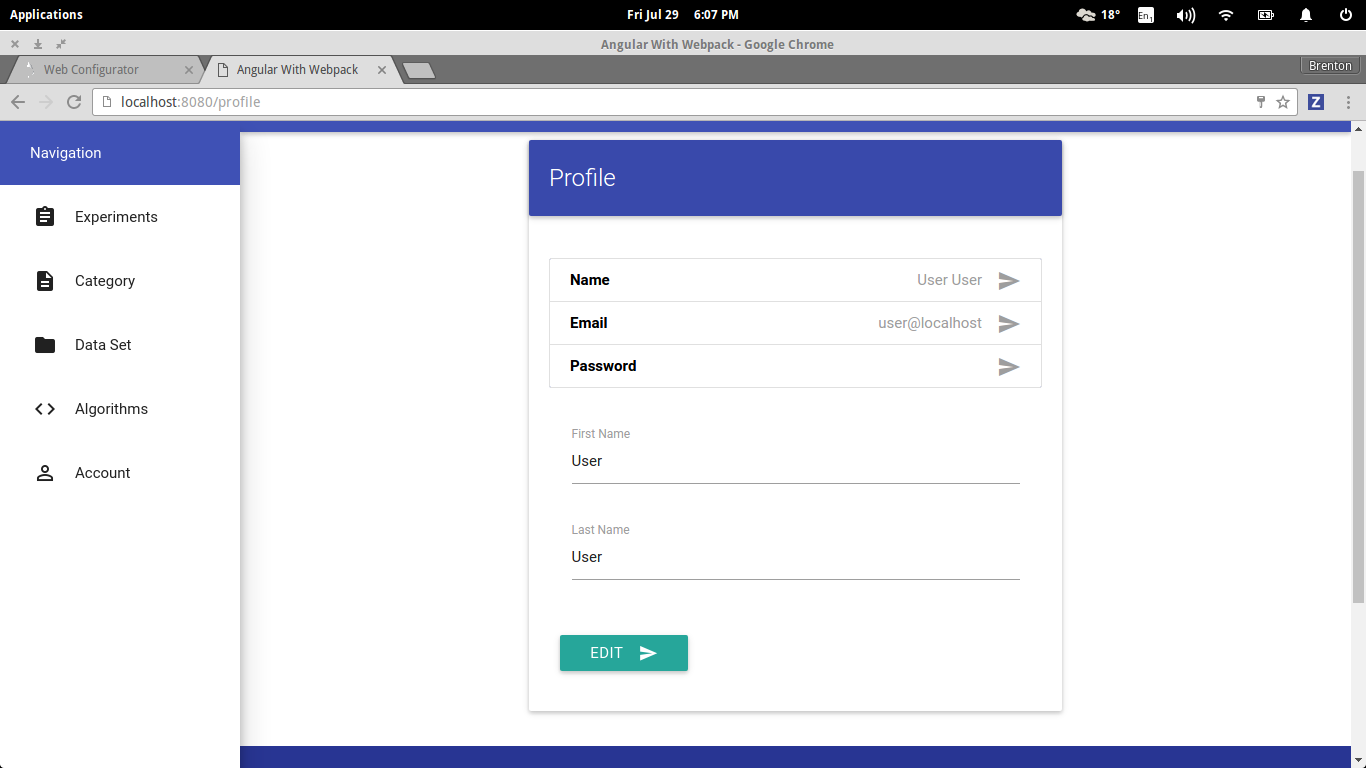
\includegraphics[scale=0.3]{../Images/User Manual/Profile Page1.png}
		\caption{Edit name}
		\label{fig:ProfilePage1}
	\end{center}  
\end{figure}
\begin{figure}[H]
	\begin{center}
		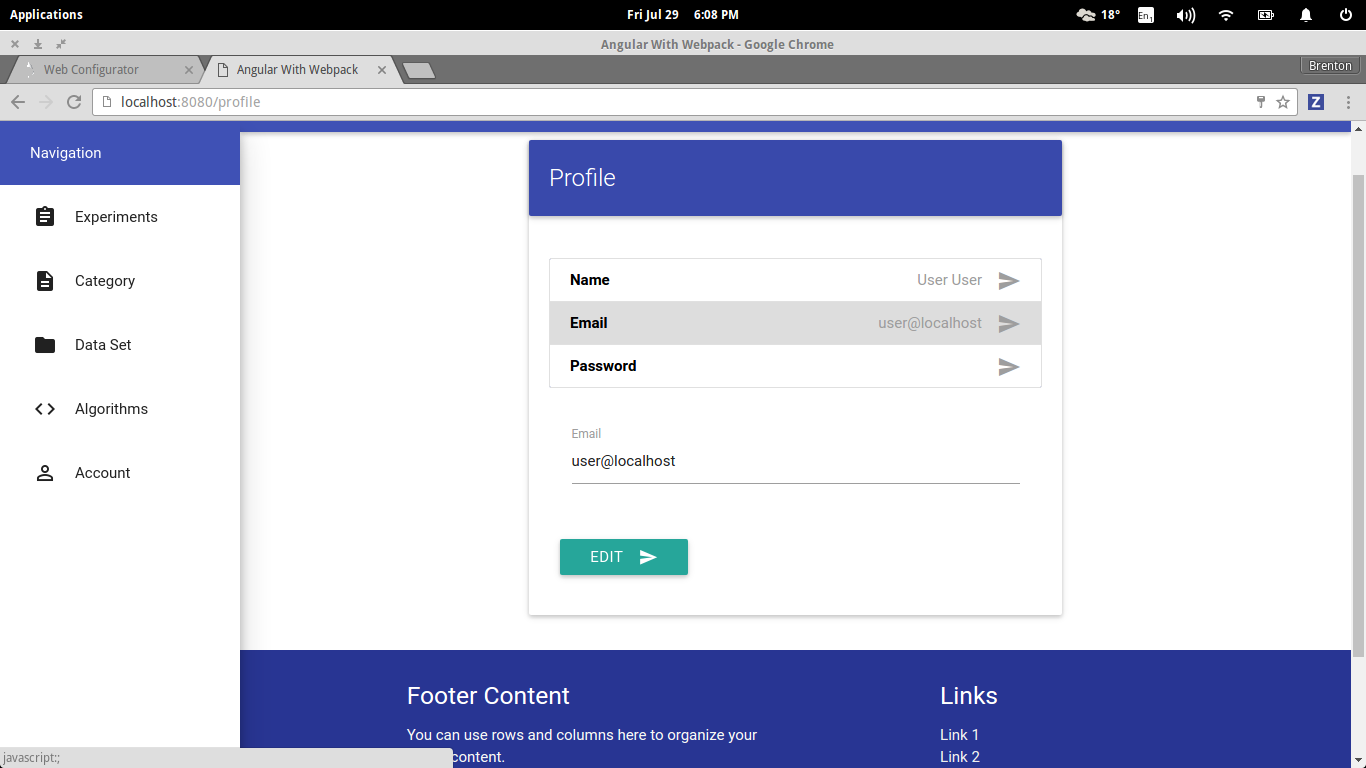
\includegraphics[scale=0.3]{../Images/User Manual/Profile Page2.png}
		\caption{Edit email}
		\label{fig:ProfilePage2}
	\end{center}  
\end{figure}
\begin{figure}[H]
	\begin{center}
		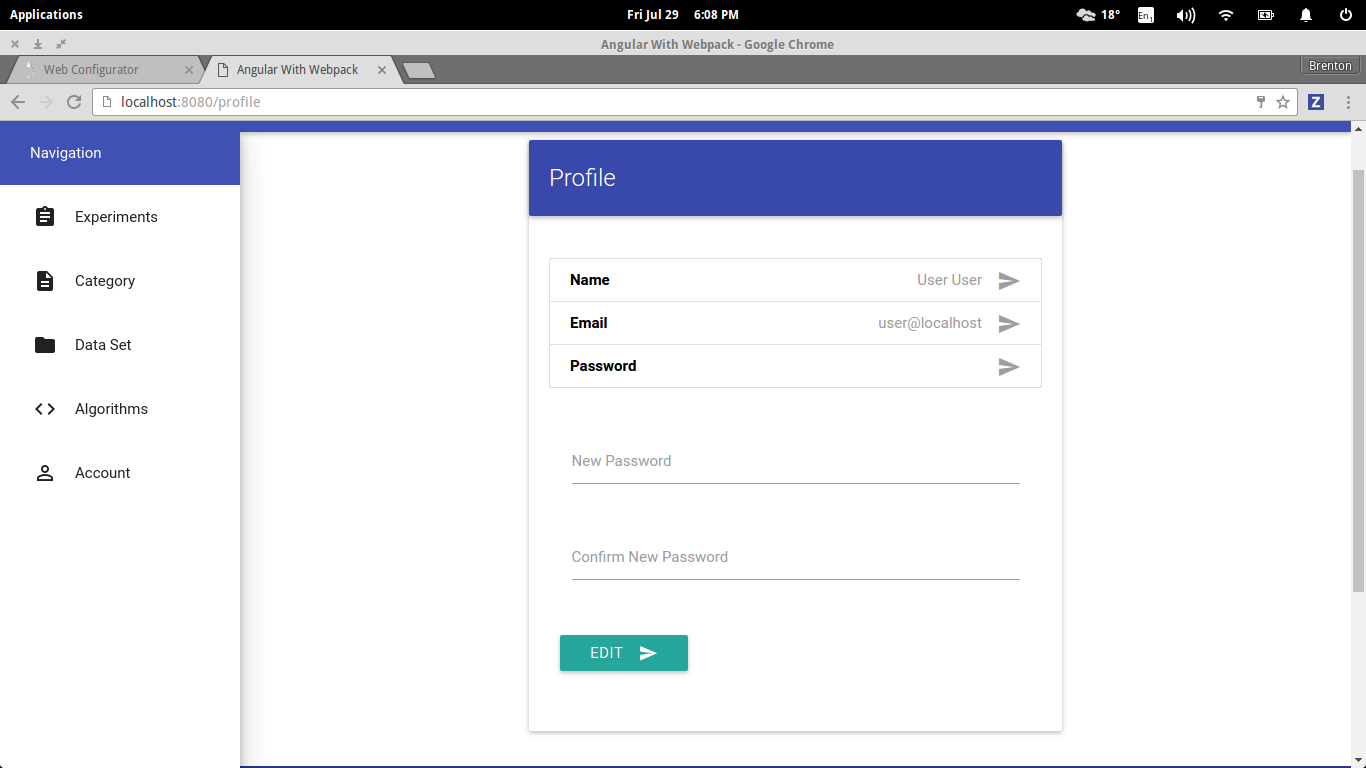
\includegraphics[scale=0.3]{../Images/User Manual/Profile Page3.png}
		\caption{Edit password}
		\label{fig:ProfilePage3}
	\end{center}  
\end{figure}
\clearpage
\section{Forgot password}
If one arrives at the landing page, and realizes they have lost or forgotten their password. They can select the
"Forgotten your password?" link at the bottom right which will take them to the page seen in Figure \ref{fig:forgotPage}.
\begin{figure}[H]
	\begin{center}
		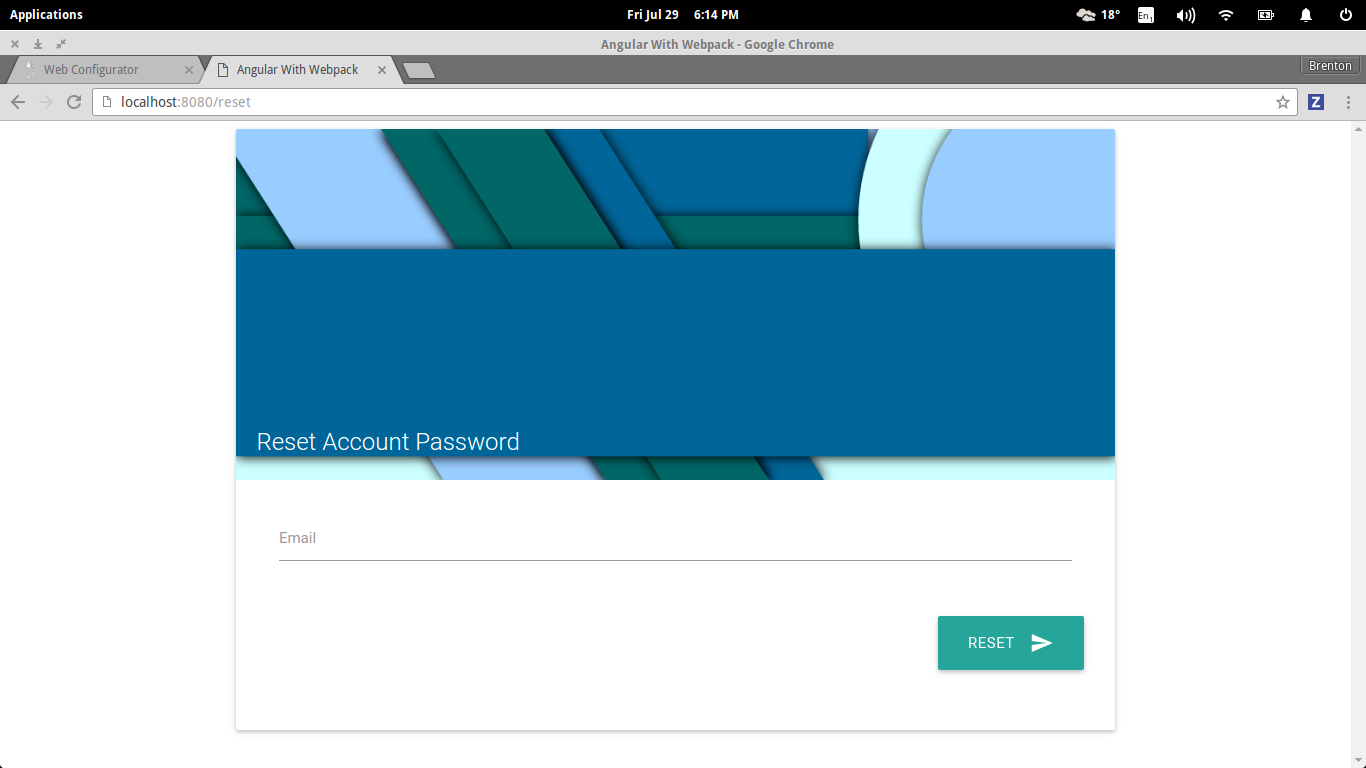
\includegraphics[scale=0.3]{../Images/User Manual/Forgot Page.png}
		\caption{Forgot password page}
		\label{fig:forgotPage}
	\end{center}  
\end{figure}
\clearpage After entering their registered email address, the user will receive an email with a link to a page to reset their password
as seen in Figure \ref{fig:resetPage}. After the user as filled in their details, the user should click "Reset".
\begin{figure}[H]
	\begin{center}
		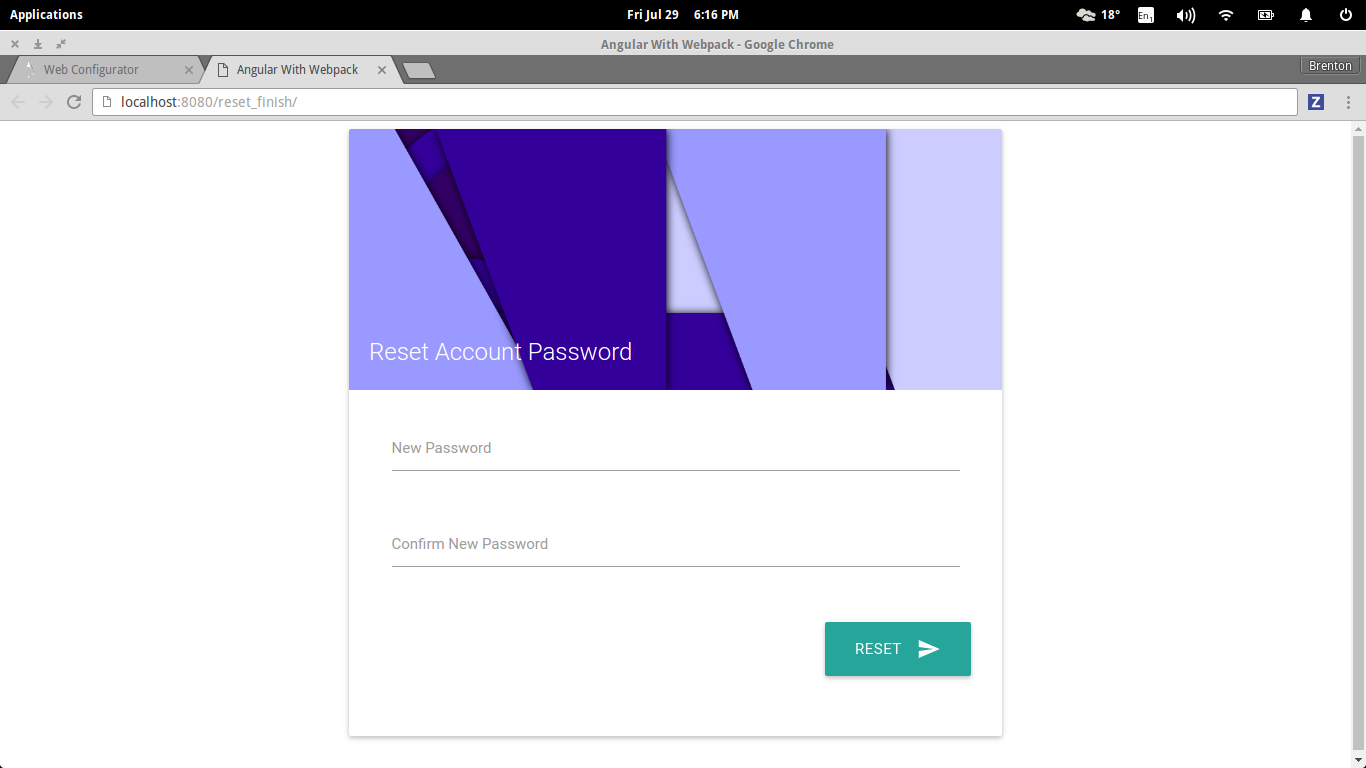
\includegraphics[scale=0.3]{../Images/User Manual/Reset Page.png}
		\caption{Reset password page}
		\label{fig:resetPage}
	\end{center}  
\end{figure}

\clearpage
\section{Experiment}
In order for a user to view their experiments the would navigate to the View Experiments
page as seen in Figure \ref{fig:viewExperiments} and a list of all current experiments 
being run or that have been run for the user will be displayed. 
\begin{figure}[H]
	\begin{center}
		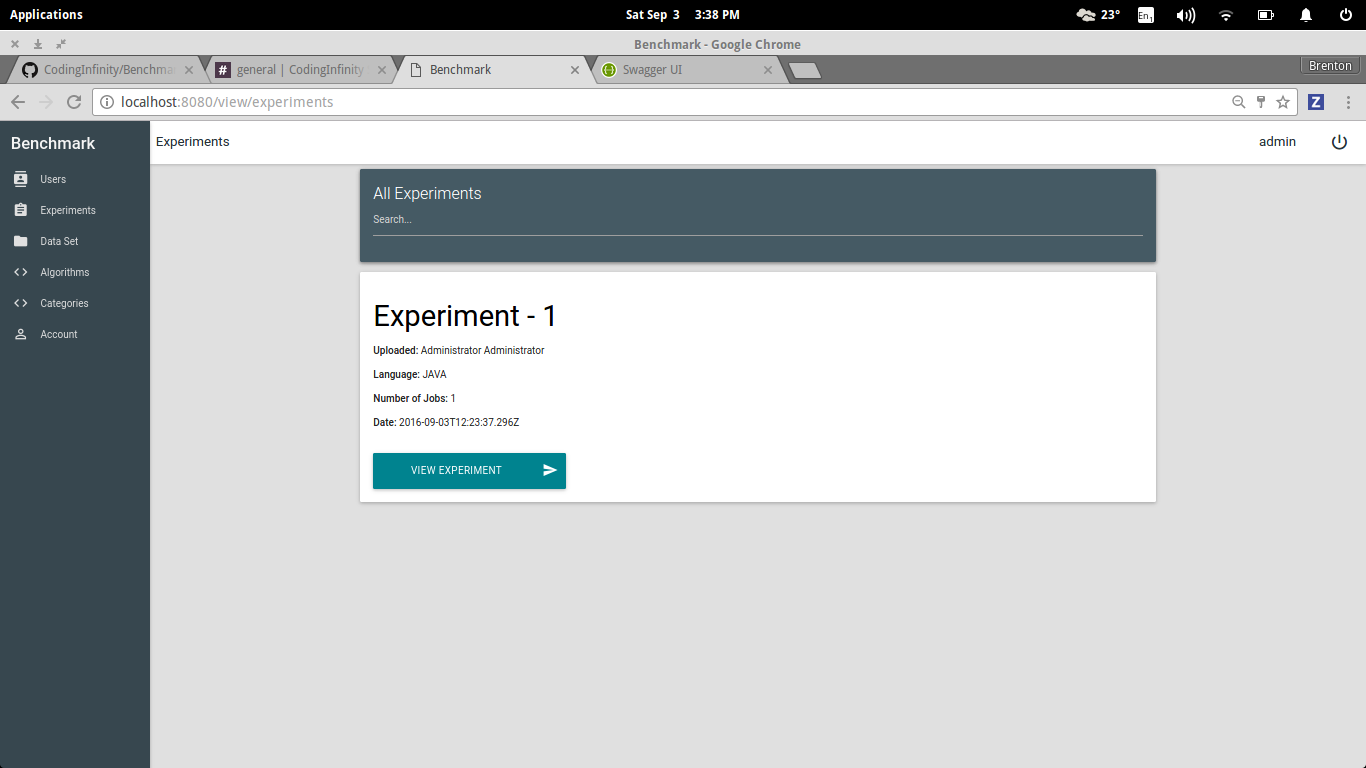
\includegraphics[scale=0.3]{../Images/User Manual/View Experiments.png}
		\caption{View Experiments page}
		\label{fig:viewExperiments}
	\end{center}  
\end{figure}
\clearpage
 The user can click on an individual experiment to see more detail surrounding the experiment
 as seen in Figure \ref{fig:viewExperiment}. If the test has finished executing a chart will
 display providing the user with a quick graphical representation of their results.
\begin{figure}[H]
	\begin{center}
		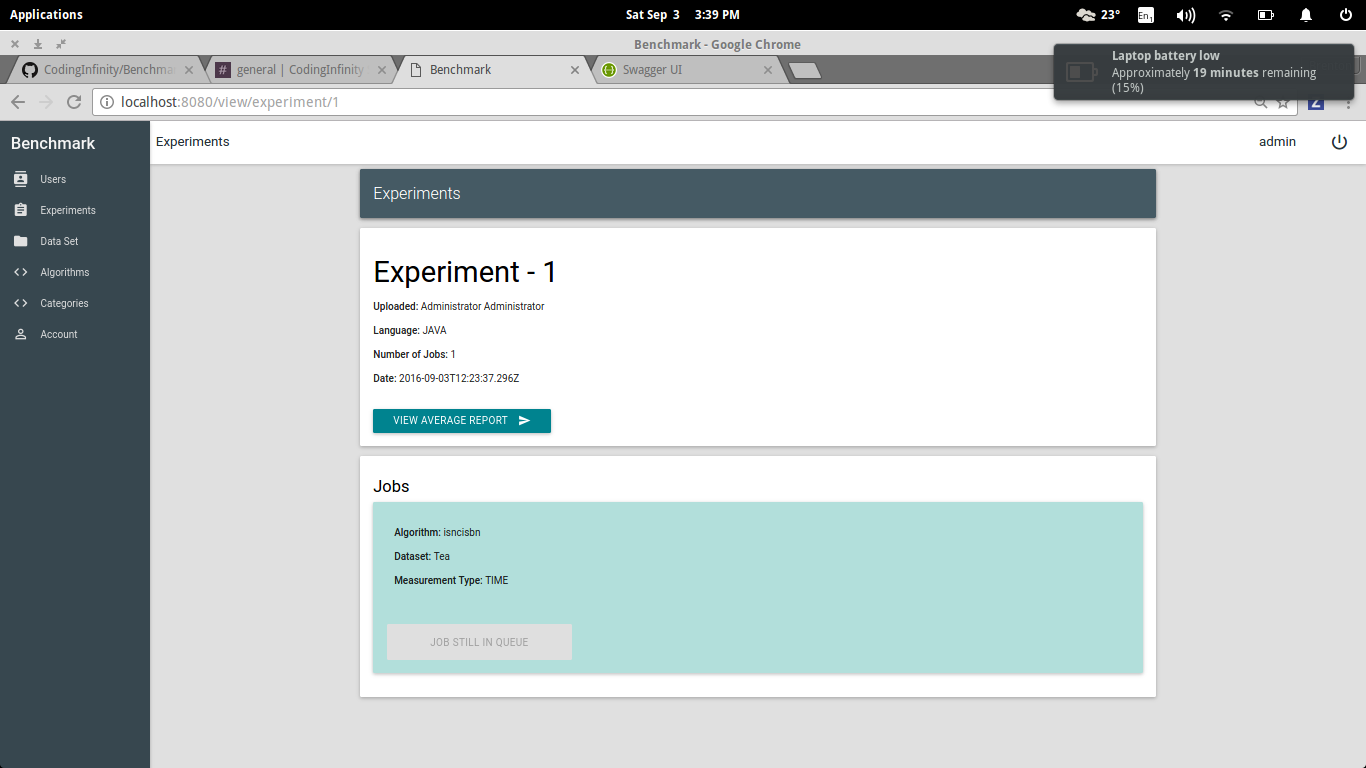
\includegraphics[scale=0.3]{../Images/User Manual/View Experiment.png}
		\caption{View experiment page}
		\label{fig:viewExperiment}
	\end{center}  
\end{figure}
\clearpage
A user can also create new experiments as seen in Figure \ref{fig:createExperiment}, 
there are a variety of customization options available to the user regarding the creation
of the experiment.

\begin{figure}[H]
	\begin{center}
		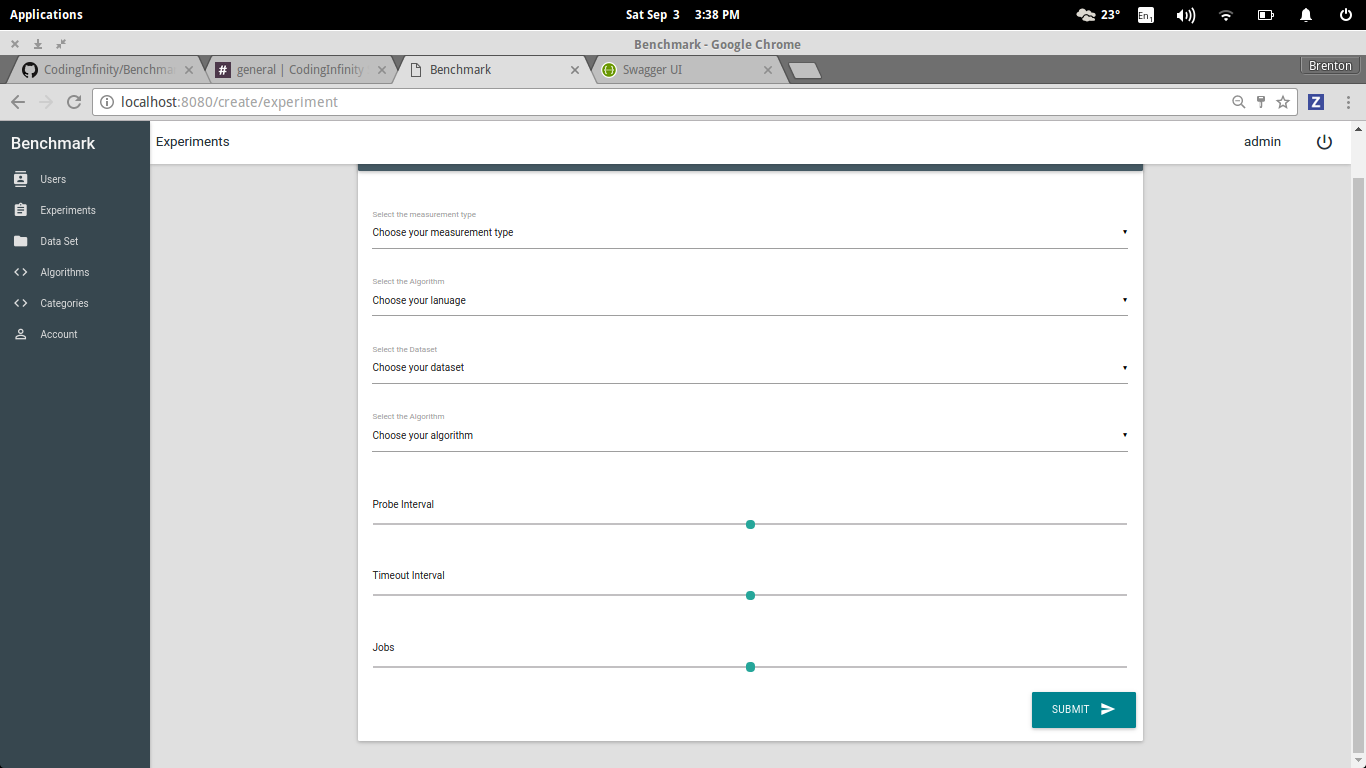
\includegraphics[scale=0.3]{../Images/User Manual/Create Experiment.png}
		\caption{Create experiment page}
		\label{fig:createExperiment}
	\end{center}  
\end{figure}

\subsection{Measurement Type}
The measurement type specifies what the user would like benchmarked. The options are
\begin{itemize}
  \item CPU - Measure CPU usuage of the application
  \item Memory - Measure the memory usuage of the application
  \item Wall Clock - Measure the time it takes an algorithm to execute
\end{itemize}

\subsection{Language}
The user will need to select the language of the application they are benchmarking.
The options are
\begin{itemize}
  \item C++
  \item Java
  \item Python
\end{itemize}


\subsection{Datasets}
The user must select all datasets the chosen algorithm must be benchmarked against. At least
one dataset must be selected.

\subsection{Algorithm}
The user must select the algorihtm that must be benchmarked.


\subsection{Probe Interval}
Value specified in seconds indicating the interval between consecutive probes. Minimal probe value is
1 with an no upper bound.

\subsection{Timeout}
The timeout specified in seconds indicating the maximum allowed time an algorithm
may run on the monitor node before it must be terminated, this is a safeguard feature.

\subsection{Jobs}
Indicates how many runs of each algorithm, dataset and measurement pairing must be scheduled.

\clearpage
\section{Category}
In order for a user to view this section they need to be logged in as an administrator.
By clicking the category drop down item in the navigation menu, the user has access to
view all algorithm categories as seen in Figure \ref{fig:viewAlCat}.

\begin{figure}[H]
	\begin{center}
		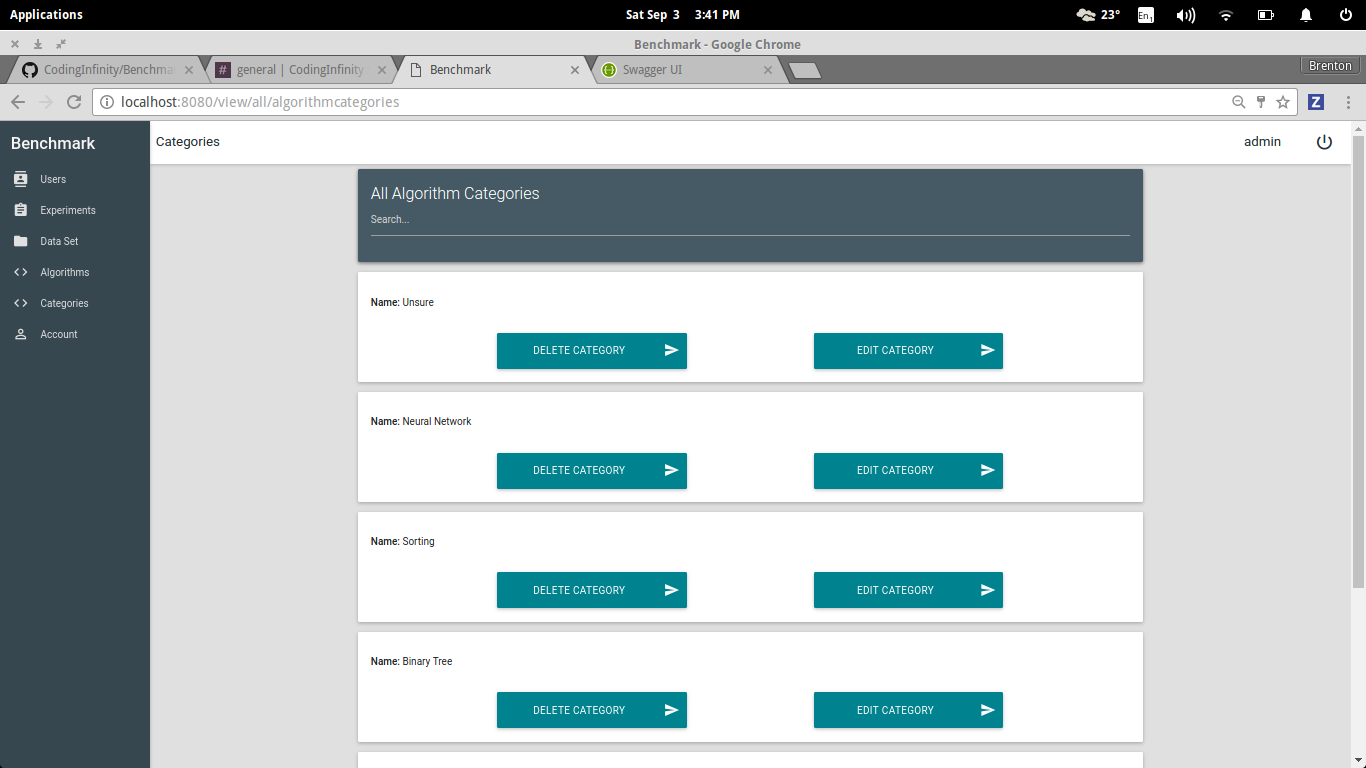
\includegraphics[scale=0.3]{../Images/User Manual/View Algorithm Categories.png}
		\caption{View all algorithm categories page}
		\label{fig:viewAlCat}
	\end{center}  
\end{figure}
\clearpage
Create new algorithm categories as seen in Figure \ref{fig:createAlCat}.
\begin{figure}[H]
	\begin{center}
		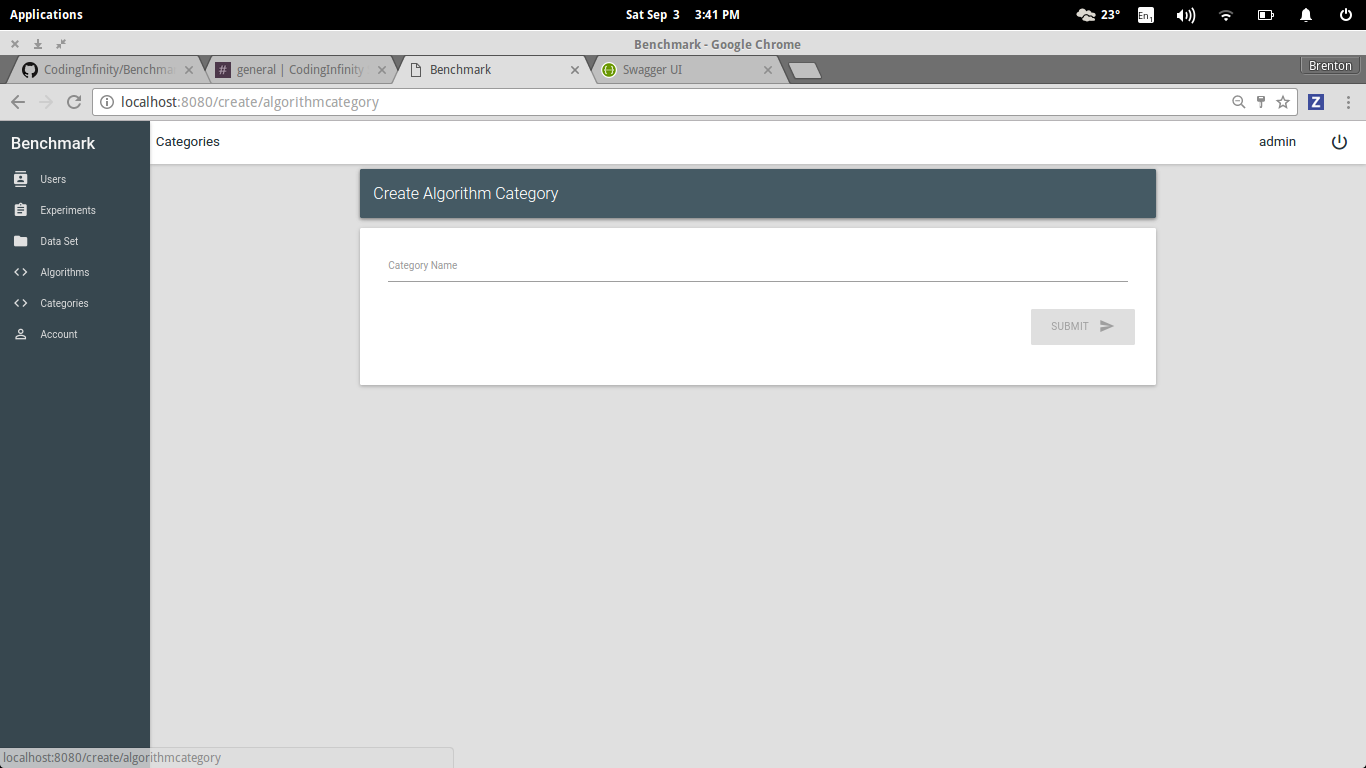
\includegraphics[scale=0.3]{../Images/User Manual/Create Algorithm Category.png}
		\caption{Create algorithm category page}
		\label{fig:createAlCat}
	\end{center}  
\end{figure}
\clearpage
View all dataset categories as seen in Figure \ref{fig:viewDataCat}
\begin{figure}[H]
	\begin{center}
		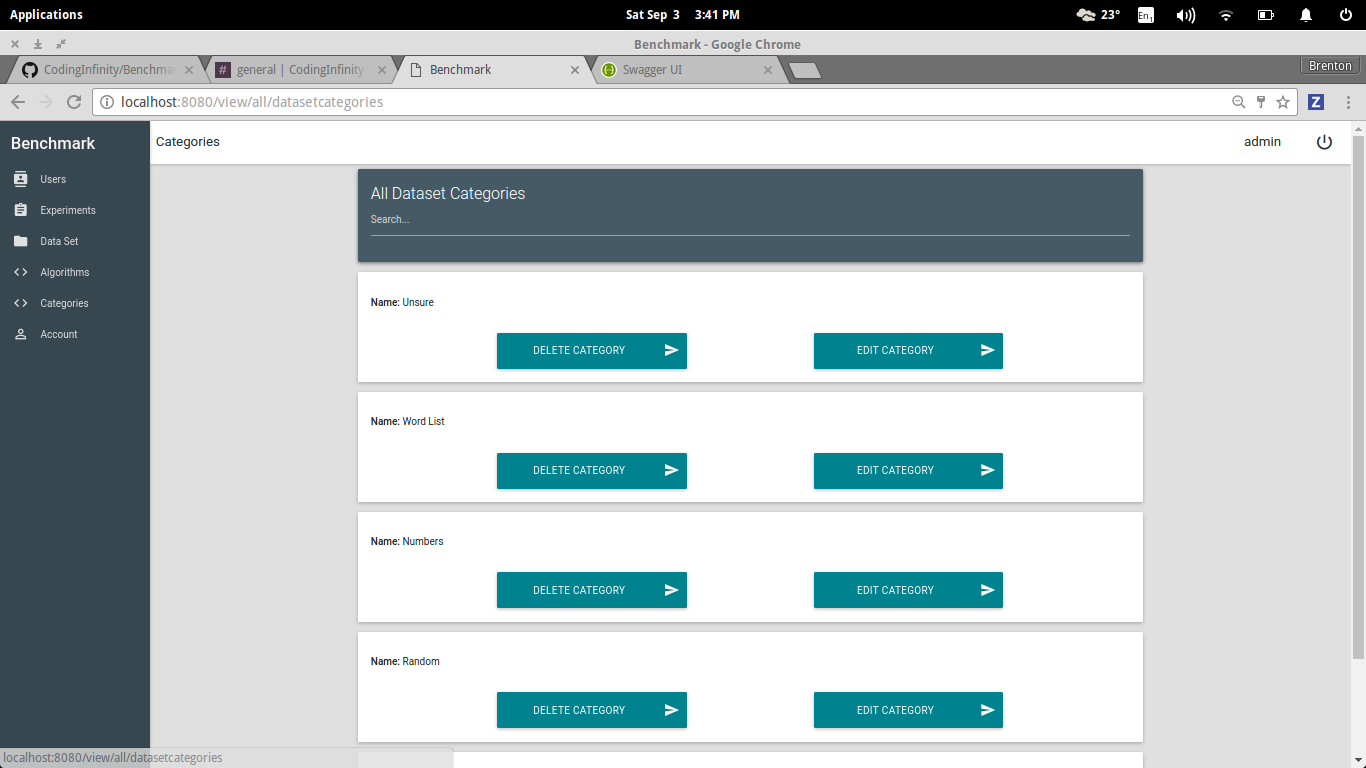
\includegraphics[scale=0.3]{../Images/User Manual/View Dataset Categories.png}
		\caption{View all dataset categories page}
		\label{fig:viewDataCat}
	\end{center}  
\end{figure}
\clearpage
Create new dataset categories as seen in Figure \ref{fig:createDataCat}.
On the respective viewing pages, a user can delete and edit certain categories.
\begin{figure}[H]
	\begin{center}
		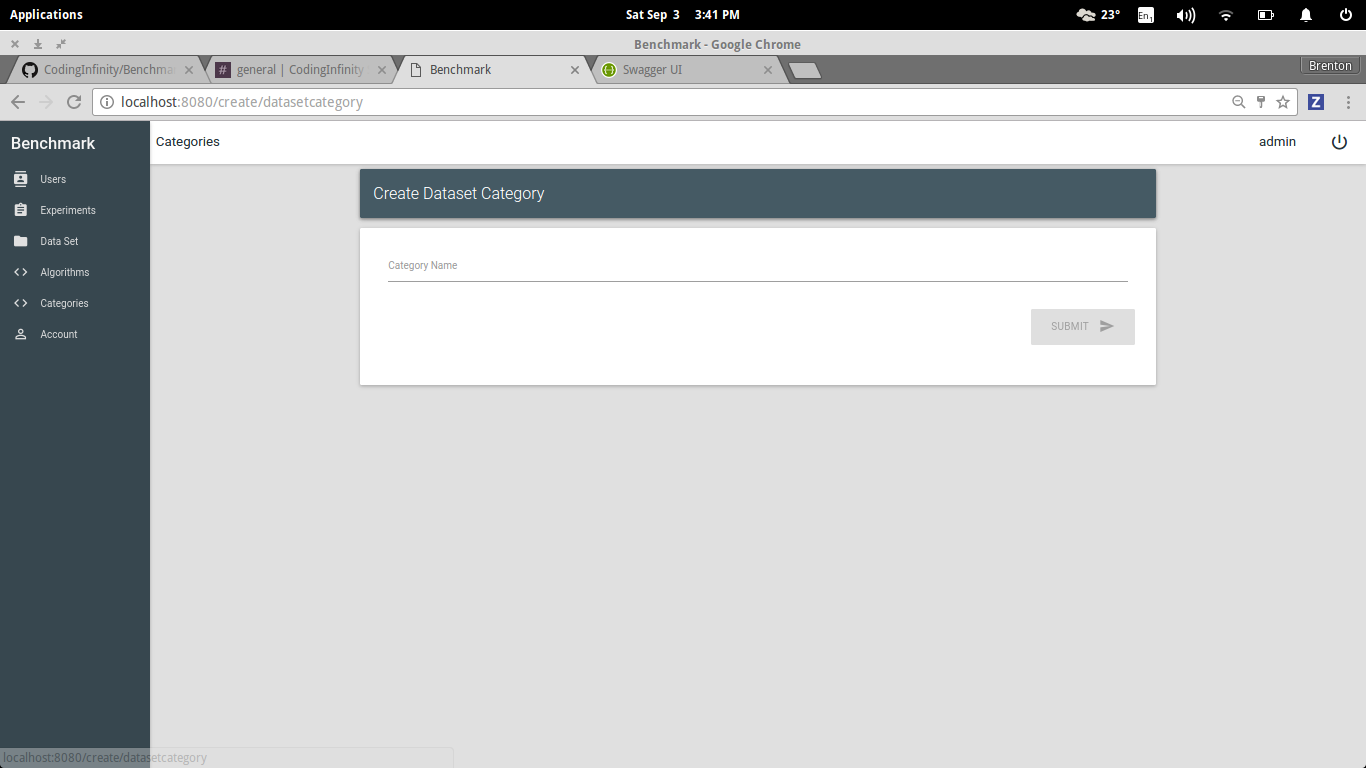
\includegraphics[scale=0.3]{../Images/User Manual/Create Dataset Category.png}
		\caption{Upload dataset category page}
		\label{fig:createDataCat}
	\end{center}  
\end{figure}

\section{Dataset}
This section can be accessed by expanding the data set item in the navigation bar, from
here a user has the ability to navigate to pages that will allow them to view all data
sets as seen in Figure \ref{fig:viewAllData}.

\begin{figure}[H]
	\begin{center}
		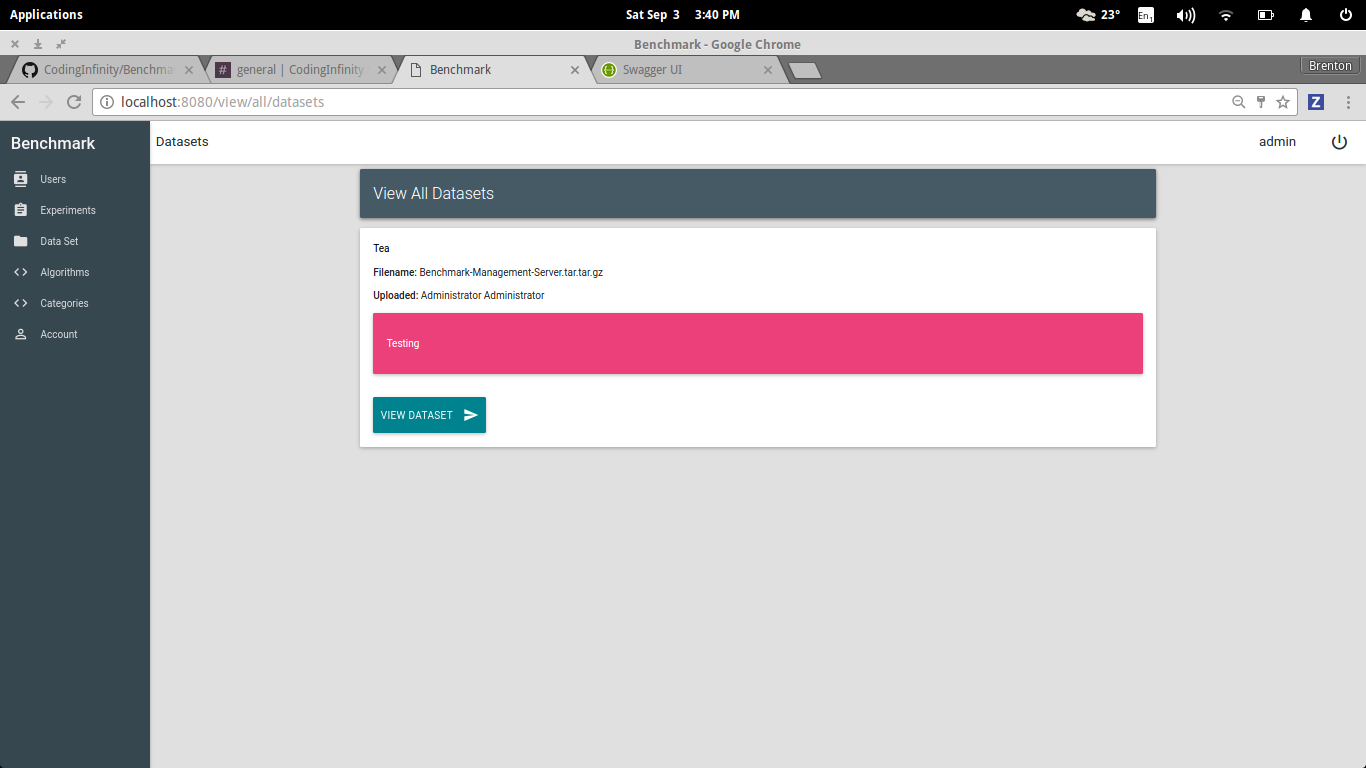
\includegraphics[scale=0.3]{../Images/User Manual/View All Datasets.png}
		\caption{View all datasets page}
		\label{fig:viewAllData}
	\end{center}  
\end{figure}
\clearpage
Simply view the data sets they have created as seen in Figure \ref{fig:viewUserData}
\begin{figure}[H]
	\begin{center}
		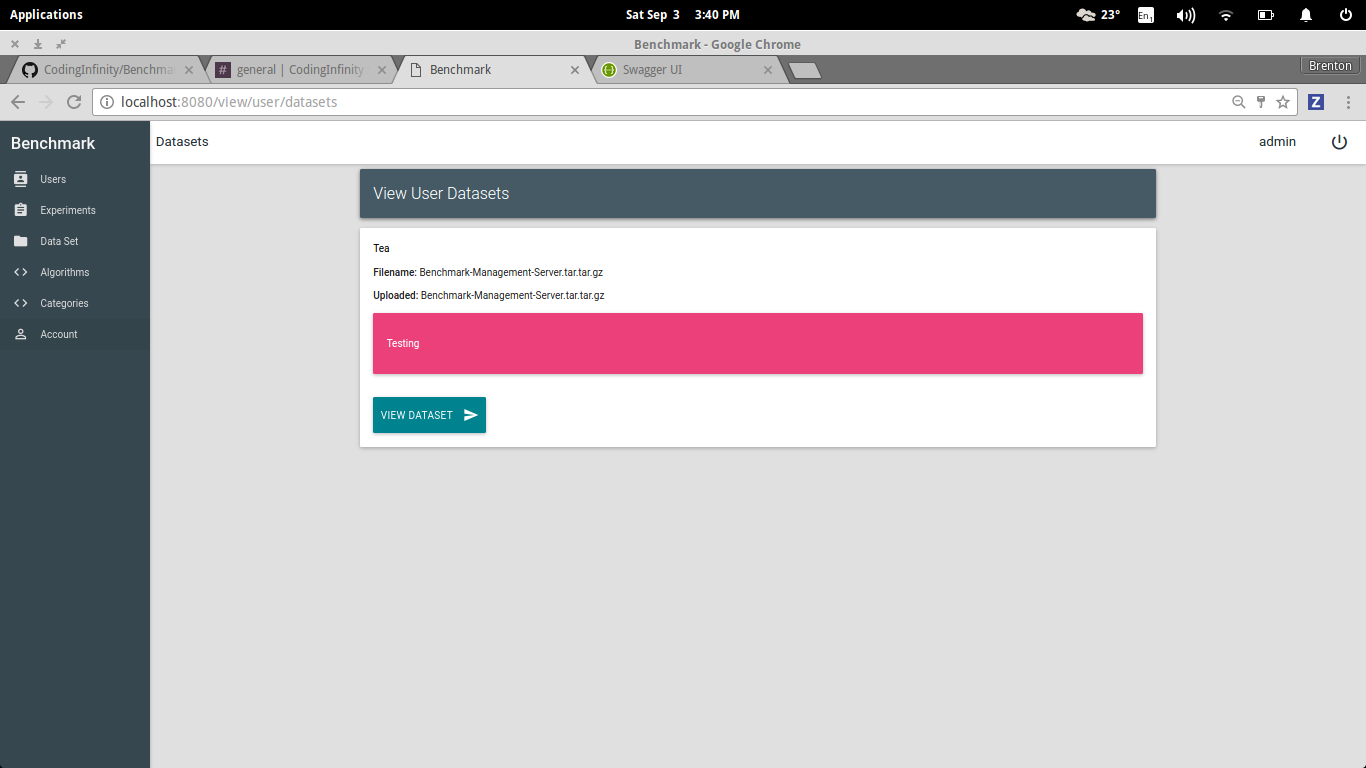
\includegraphics[scale=0.3]{../Images/User Manual/View User Datasets.png}
		\caption{View user datasets page}
		\label{fig:viewUserData}
	\end{center}  
\end{figure}
\clearpage 
From either of the above mentioned pages they can choose to view the data set in more
detail as seen in \ref{fig:viewData}
\begin{figure}[H]
	\begin{center}
		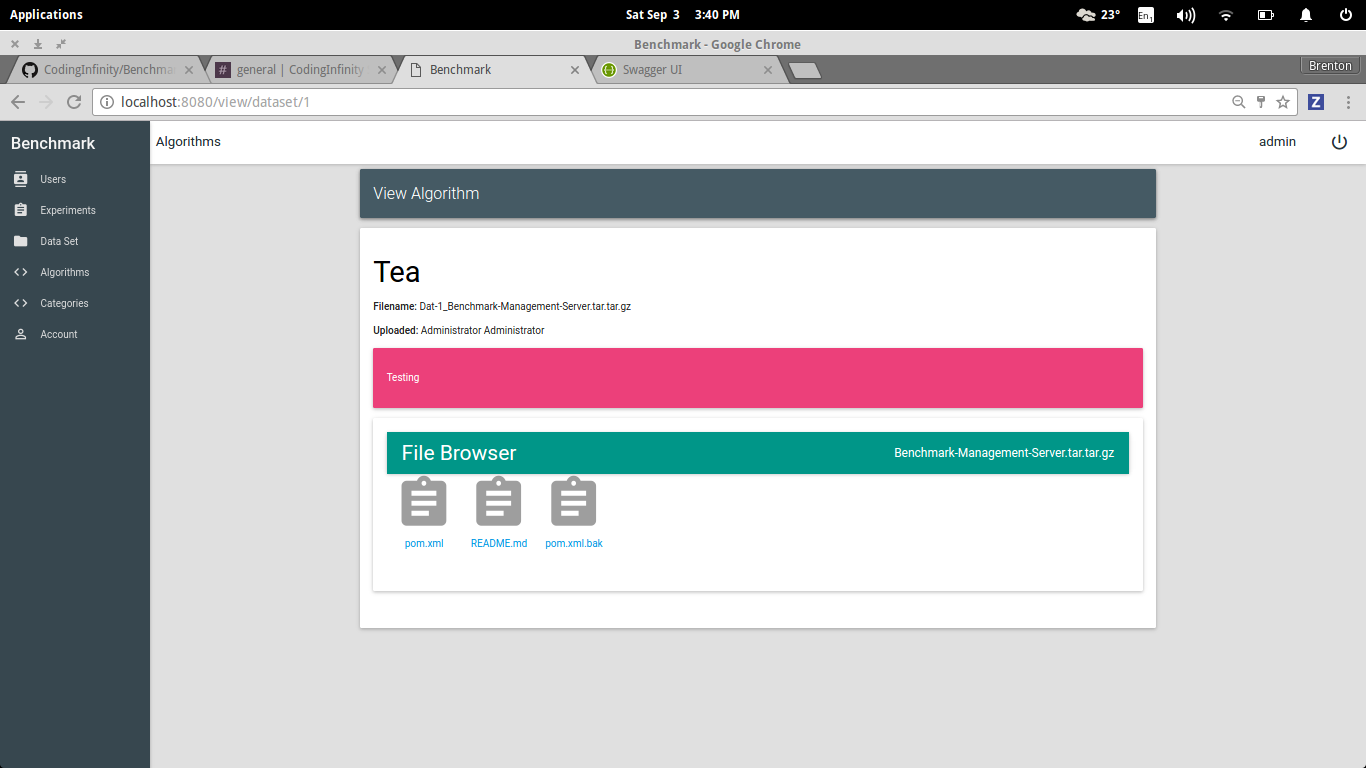
\includegraphics[scale=0.3]{../Images/User Manual/View Dataset.png}
		\caption{View dataset page}
		\label{fig:viewData}
	\end{center}  
\end{figure}
\clearpage
Or they can upload a new data set as seen in Figure \ref {fig:createData}.
\begin{figure}[H]
	\begin{center}
		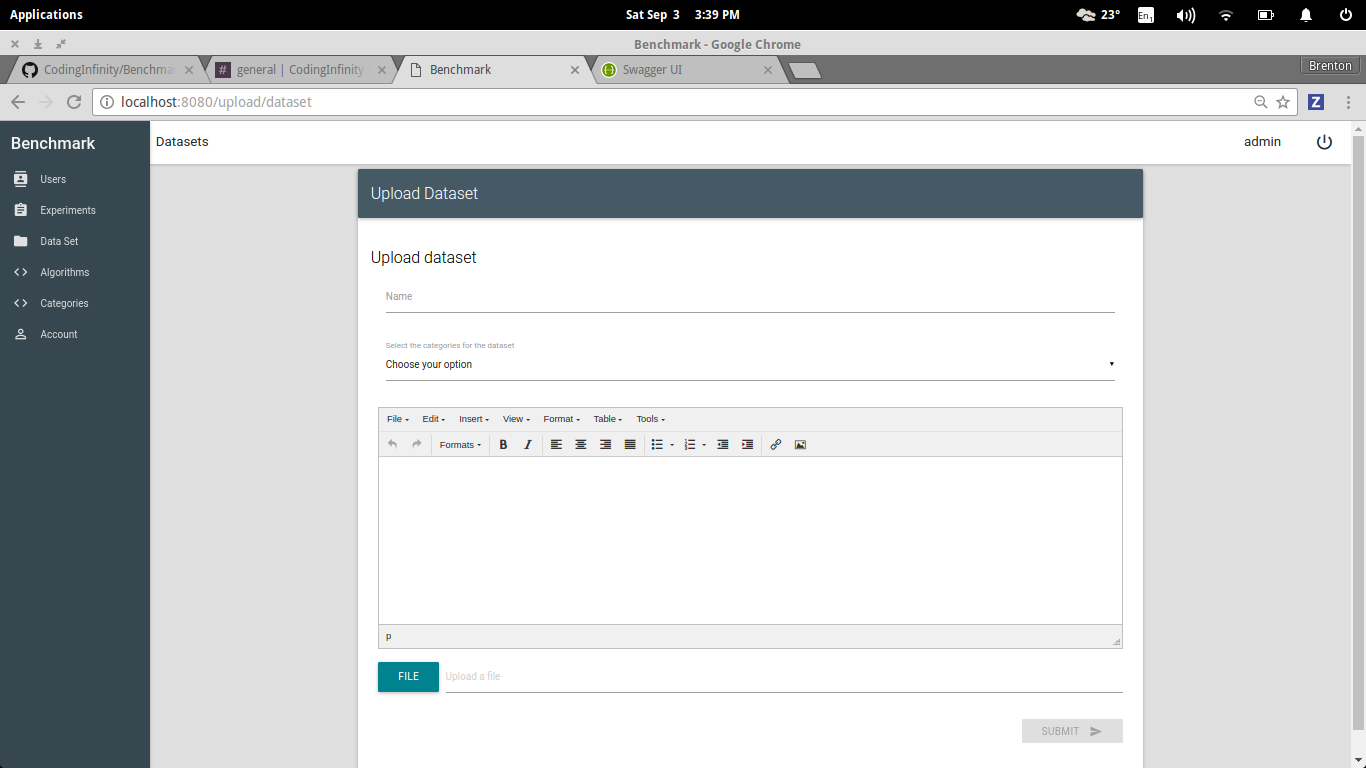
\includegraphics[scale=0.3]{../Images/User Manual/Upload Dataset.png}
		\caption{Create dataset page}
		\label{fig:createData}
	\end{center}  
\end{figure}
\clearpage
\section{Algorithms}
This section is mutatuis mutandis as the Dataset section. See above mentioned section and figures.
\end{document}
